\chapter{Python 中的 Numpy 与 Pandas}

\section{Numpy 的常用操作}

\clearpage
\section{Pandas 的常用操作}

Pandas 是 Python 做统计分析时最重要的数据分析工具之一,它基于 Numpy 开发,提供了许多处理大型数据集所需的函数,可以灵活高效的处理各种数据集。

Pandas 一般使用两种数据类型:DataFrame 和 Series。其中 DataFrame 是二维数据,而 Series 是一维数据。可以这样简单理解:DataFrame 相当于 Excel 里面的一张表,而 Series 是表中的某一列。还有一个表示三维数据的类型 Panel,但我们经常使用的是前面两种数据类型。使用 Pandas 时首先到导入 pandas 包。

\begin{lstlisting}[Language=Python]
import pandas as pd
\end{lstlisting}

\subsection{创建、读取和存储数据}

\subsubsection{创建}
 例如有下面的数据:

 \begin{table}[!ht]
 \centering
 \renewcommand{\arraystretch}{1.2}
 \begin{tabular}{|l|l|l|l|}
 \hline
 &统计学 & 高数 & 英语 \\ \hline
 张三 & 85 & 82 & 84 \\ \hline
 李四 & 68 & 63 & 90 \\ \hline
 王五 & 90 & 88 & 78 \\ \hline
 \end{tabular}
 \end{table}

我们可以使用下面的代码读取到一个 DataFrame 里面:

\begin{lstlisting}[Language=Python]
df = pd.DataFrame({'统计学': [85, 68, 90], '高数': [82, 63, 88], '英语': [84, 90, 78]}, index=['张三', '李四', '王五'])
print(df)
\end{lstlisting}

从上面可以看出,DataFrame 通过一个字典类型设置各列的标题及对应数值,通过一个 index 数组设置行标题。还有一种方式是通过 numpy 的 array 数组设置数值,然后通过 columns 数组设置列标题,通过 index 数组设置行标题\footnote{如果创建时不设置行标题或列标题,系统会自动生成从 0 到行数或列数的数组作为标题}:

\begin{lstlisting}[Language=Python]
import numpy as np

df = pd.DataFrame(np.array([[85, 68, 90], [82, 63, 88], [84, 90, 78]]), columns=['统计学', '高数', '英语'], index=['张三', '李四', '王五'])
print(df)
\end{lstlisting}

一个 DataFrame 包括 columns(列标题),index(行标题)与 values(数值)三个部分,上述例子中的 columns, index,values 如下图所示:

\begin{figure}[!ht]
\centering
  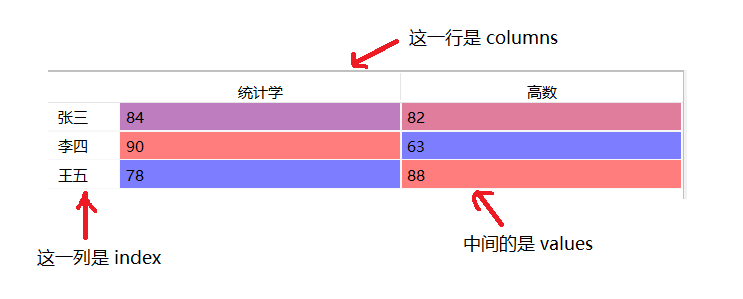
\includegraphics{figure/chapter2/pandas.png}
\end{figure}

\subsubsection{读取}
大部分情况下,我们要读取 Excel 里面的数据,假设上面的例子在 excel 文件 '成绩数据.xlsx' 并放在电脑硬盘某个位置:

\begin{figure}[!ht]
\centering
  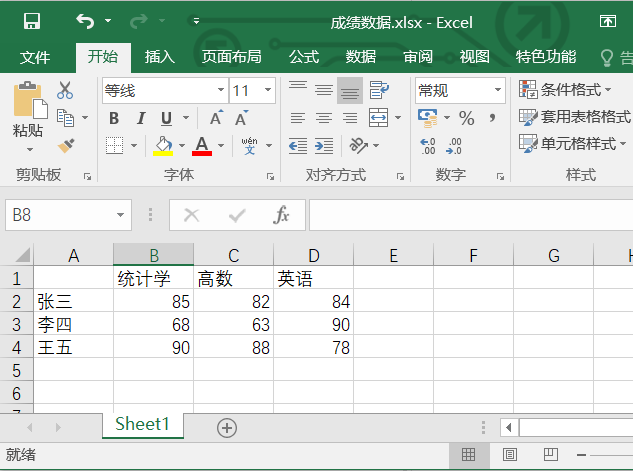
\includegraphics[scale=0.7]{figure/chapter2/pandas2.png}
\end{figure}

可以通过下面的代码读取文件:

\begin{lstlisting}[Language=Python]
df = pd.read_excel(r'D:\Users\chen_\git\Statistics-book\datas\成绩数据.xlsx', index_col=0)
\end{lstlisting}

数据文件的地址位于 \path{`D:\Users\chen_\git\Statistics-book\datas\成绩数据.xlsx'},使用 read\_excel 时\textbf{在文件位置字符串前面加上字母 r},这样 python 就能找到我们的数据文件了。index\_col=0 表示行标题位于第一列(不然 read\_excel 会把第一列内容读取到 values 里面,并默认 index 为 0, 1, 2, \dots)。read\_excel 会自动将 Excel 第一行的内容作为行标题。read\_excel 的一般语法为:

\begin{center}
\begin{tcolorbox}[title = read\_excel 函数的语法]
\textbf{read\_excel(io, sheetname=0, header=0, skiprows=None,  index\_col=None)}
\tcblower
\vspace{10pt}

\begin{tcboutputlisting}
\begin{tabular}{>{\bfseries}ll}
  io &数据文件的地址与名字,一般为字符串\\
  sheetname & 工作簿名字,默认为0,表示读取第一张工作簿\\
header &作为列名的行,默认为0,即取第一行的值为列名\\
skiprows&省略指定行数的数据,从第一行开始查起\\
index\_col&行标题所在的列\\
\end{tabular}
\end{tcboutputlisting}
\tcbuselistingtext

\end{tcolorbox}
\end{center}

\sloppy
更多的语法设置可以查看官网文档:

\href{https://pandas.pydata.org/pandas-docs/version/0.20/generated/pandas.read\_excel.html}{https://pandas.pydata.org/pandas-docs/version/0.20/generated/pandas.read\_excel.html}

还有一种常见的数据文件类型为 csv,我们只需使用 pandas 中的函数 read\_csv,它的语法与 read\_excel 基本一样。但是, read\_csv 可以读取网络数据库中的 csv 文件,例如下面的例子显示世界上所有国家与所属的大洲。

\begin{lstlisting}[Language=Python]
df = pd.read_csv('https://raw.githubusercontent.com/cs109/2014_data/master/countries.csv')
print(df)
\end{lstlisting}

\begin{figure}[!ht]
\centering
  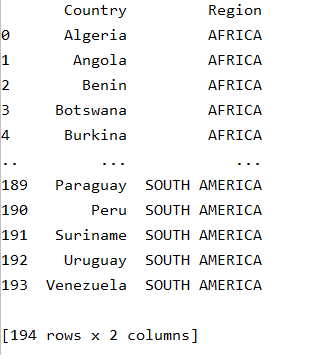
\includegraphics[scale=0.7]{figure/chapter2/pandas7.png}
\end{figure}
\subsubsection{存储}

存储时使用函数 to\_excel 或 to\_csv。例如我们将 DataFrame 存储到 \path{E:\datas} 文件夹里,并命名为 marks.xlsx:

\begin{lstlisting}[Language=Python]
import pandas as pd
import numpy as np

df = pd.DataFrame(np.array([[85, 68, 90], [82, 63, 88], [84, 90, 78]]), columns=['统计学', '高数', '英语'], index=['张三', '李四', '王五'])
df.to_excel(r'E:datas\marks.xlsx')
\end{lstlisting}

在上面的代码中,若直接写成 df.to\_excel('marks.xlsx'),则文件存储的路径为当前工作环境所在的文件夹。


\subsection{查看数据}

\subsubsection{概览数据}
快速查看 DataFrame 各列数据的统计信息可以使用 discribe() 函数,包括各列数据的非空数值数目、均值、标准差、最大值、最小值、分位数。例如上面的例子:

\begin{lstlisting}[Language=Python]
df.describe()
\end{lstlisting}

\begin{figure}[!ht]
\centering
  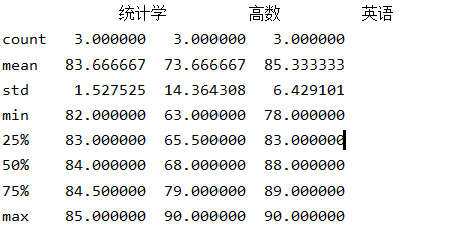
\includegraphics[scale=0.7]{figure/chapter2/pandas3.png}
\end{figure}

info() 函数可以查看各列数据的类型:

\begin{lstlisting}[Language=Python]
df.info()
\end{lstlisting}

\begin{figure}[!ht]
\centering
  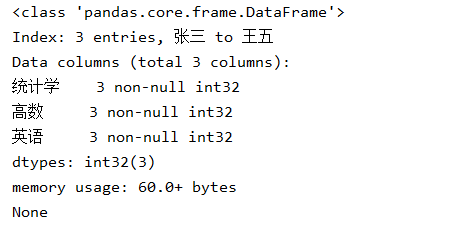
\includegraphics[scale=0.8]{figure/chapter2/pandas4.png}
\end{figure}

DataFrame 的 sample() 函数可以从数据中随机抽取样本,小括号中用数字表示抽取的样本个数。例如,下面的代码从 df 里面随机抽取 2 个样本:
\begin{lstlisting}[Language=Python]
df.sample(2)
\end{lstlisting}

\begin{figure}[!ht]
\centering
  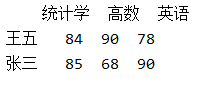
\includegraphics[scale=0.8]{figure/chapter2/pandas8.png}
\end{figure}

另外,head() 函数可以显示 DataFrame 前五行数据,而 tail() 函数可以显示 DataFrame 最后五行数据。

\subsubsection{查看单列、单行、单元格数据}

查看某一列数据时,最简单的方式是中括号里面输入列名的方式,例如查看英语成绩那一列数据:
\begin{lstlisting}[Language=Python]
df['英语']
\end{lstlisting}

\begin{figure}[!ht]
\centering
  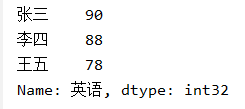
\includegraphics[scale=0.8]{figure/chapter2/pandas5.png}
\end{figure}

查看某一行数据时,最简单的方式是中括号里面输入行名方式,例如查看张三哪一行的数据:
\begin{lstlisting}[Language=Python]
df['张三']
\end{lstlisting}

也可以用中括号里面跟着行索引的方式(行数 : 行数 + 1),即 df[0:1],与上面代码显示效果一样。


\begin{figure}[!ht]
\centering
  
\includegraphics[scale=0.8]{figure/chapter2/pandas6.png}
\end{figure}


若查看某个单元格,比较方便的方式是用两个中括号,每个中括号内分别跟着行名和列名,例如查看张三的高数成绩:
\begin{lstlisting}[Language=Python]
df['张三']['高数']  # 显示张三的高数成绩为 68
\end{lstlisting}



\subsubsection{查看多列、多行数据 iloc}

查看多行、多列数据时,一般用 iloc 比较方便,而且 iloc 不仅能查看多行多列数据,也能查看单行、单列或某个单元格数据:

例如,查看行:

\begin{lstlisting}[Language=Python]
df.iloc[1]          # 查看第 2 行数据
df.iloc[0:2]        # 查看前 2 行数据
df.iloc[[0, 2]]     # 查看第 1 行与第 3 行数据
\end{lstlisting}

查看列:

\begin{lstlisting}[Language=Python]
df.iloc[:, 1]       # 查看第 2 列数据
df.iloc[:, 0:2]     # 查看前 2 列数据
df.iloc[:, [0, 2]]  # 查看第 1 列与第 3 列数据
\end{lstlisting}

查看一块数据:
\begin{lstlisting}[Language=Python]
df.iloc[0:2, 0:2]          # 查看前 2 行,前 2 列的一块数据
df.iloc[[0, 2],  [0, 2]]   # 查看第 1、第 3 行,第 1、第 3 列的一块数据
df.iloc[0:2, [0, 2]]       # 查看前 3 行,第 1、第 3 列的一块数据
df.iloc[[0, 2], 0:2]       # 第 1、第 3 行,前 2 列的一块数据
\end{lstlisting}

查看某个单元格:
\begin{lstlisting}[Language=Python]
df.iloc[1, 1]   # 查看第 2 行,第 2 列的单元格数据
\end{lstlisting}

\subsection{增加、删除、修改、查询数据}

\subsection{数据合并}

\subsection{数据排序}

\subsection{分组汇总数据}

\section{数据的概括性度量}
